\documentclass[hidelinks,12pt,a4paper,final]{extreport}
\usepackage[utf8]{inputenc}
\usepackage{amsmath}
\usepackage{bm}
\usepackage{amsfonts}
\usepackage{fancyhdr}
\usepackage[algo2e]{algorithm2e} 
\usepackage{amssymb}
\usepackage{float}
\usepackage{placeins}
\usepackage{graphicx}
\usepackage{hyperref}
\usepackage{url}
\usepackage[left=2.5cm,right=2.5cm,top=2cm,bottom=2cm]{geometry}
\linespread{1.2}
\usepackage{setspace}
\usepackage{titlesec}
\usepackage[yyyymmdd]{datetime}

\usepackage{times}
\renewcommand{\bibname}{REFERENCES}
\usepackage{enumerate}
\usepackage{etoolbox}
\patchcmd{\chapter}{plain}{empty}{}{}

\usepackage{tocloft,calc}
\renewcommand{\cftchappresnum}{\chaptername\space}
\setlength{\cftchapnumwidth}{\widthof{\textbf{Appendix~999~}}}
\makeatletter
\g@addto@macro\appendix{%
  \addtocontents{toc}{%
    \protect\renewcommand{\protect\cftchappresnum}{\appendixname\space}%
  }%
}
\makeatother

\titleformat{\chapter}[display]
{\normalfont\rmfamily\large\bfseries}
{\chaptertitlename\ \thechapter \centering }{16pt}{\centering \huge\uppercase}
\renewcommand{\chaptername}{CHAPTER}{\Large}
\titleformat{\section}
{\normalfont\rmfamily\normalsize\bfseries}
{\thesection}{14pt}{\large}

 \titleformat{\subsection}
{\normalfont\rmfamily\small\bfseries}
{\thesubsection}{12pt}{\normalsize} 

 \titleformat{\subsubsection}
{\normalfont\rmfamily\small\bfseries}
{\thesubsection}{12pt}{\normalsize} 

\titlespacing{\chapter}{0pc}{0pc}{0.5pc}
\titlespacing{\section}{0pc}{.5pc}{0pc}
\titlespacing{\subsection}{0pc}{1pc}{0pc}
\thispagestyle{empty}


\author
{   \textbf{Ganesh Sekhar (CHN16CS055)}\\
    \textbf{Shan Eapen Koshy (CHN16CS095)} \\[0.1mm]
	\textbf{Sachin Sajan Punoose (CHN16CS092)} \\[0.1mm]
	\textbf{S Hemanth (CHN16CS098)} \\[0.1mm]
	\textbf{to}\\
 }
\title{{\Large\textbf{Generating Usability Reports from User Inputs and Eye Movements}} \\
\vspace{1.2cm}	{\large\textbf{A PROJECT REPORT}}\\[0.2cm]
	{\small submitted by}
		}
\date{\begin{center}
\begin{small}
The APJ Abdul Kalam Technological University\\
in partial fulfillment of the requirements for the award of the Degree\\[0.2cm]
of\\[0.2cm]
Bachelor of Technology\\[0.2cm]
In\\[0.2cm]
\textit{Computer Science and Engineering}\\\end{small}
\begin{figure}[h]	
\begin{center}

\includegraphics[scale=0.3]{ceclogo.png} \\[.1cm]
\end{center}
\end{figure}
	\textbf{ Department of Computer Science and Engineering} \\
	 College of Engineering, Chengannur, Kerala -689121\\	
	July 2020\end{center}
}	

\begin{document}
\pagenumbering{gobble}
\clearpage\maketitle

\section*{\begin{center} \fontsize{14}{17} \selectfont \textbf{DECLARATION}\end{center}}
\begin{quote}

We undersigned hereby declare that the project report "Generating Usability Reports from User Inputs and Eye Movements", submitted for partial fulfillment of the requirements for the award of degree of Bachelor of Technology of the APJ Abdul Kalam Technological University, Kerala is a bonafide work done by us under supervision of Ms.Angel, Assistant Professor. This submission represents our ideas in our own words and where ideas or words of others have been included, We have adequately and accurately cited and referenced the original sources. We also declare that we have adhered to ethics of academic honesty and integrity and have not misrepresented or fabricated any data or idea or fact or source in my submission. We understand that any violation of the above will be a cause for disciplinary action by the institute and/or the University and can also evoke penal action from the sources which have thus not been properly cited or from whom proper permission has not been obtained. This report has not been previously formed the basis for the award of any degree, diploma or similar title of any other University.

\begin{tabbing}
\hspace{8.8cm}\=\kill
Place: CHENGANNUR  \> Ganesh Sekhar \\  Date:\today  \>Shan Eapen Koshy \\ \hspace{8.8cm} Sachin Sajan Punnoose \\ \hspace{8.8Cm} S Hemanth
\end{tabbing} 
\end{quote}
\newpage
\clearpage
\thispagestyle{empty}

\begin{center}\fontsize{14}{17} \selectfont \textbf{DEPARTMENT OF COMPUTER SCIENCE AND ENGINEERING}\end{center}
\begin{center}\fontsize{14}{17} \selectfont \textbf{COLLEGE OF ENGINEERING,CHENGANNUR}\end{center}
%\begin{center}\fontsize{14}{17} \selectfont \textbf{PALAKKAD}\end{center}
\begin{figure}[h]
	\begin{center}
		
\includegraphics[scale=.33]{ceclogo.png}
		\vspace{.1 cm}
	\end{center}
\end{figure}

\begin{center}\fontsize{14}{17} \selectfont \textbf{CERTIFICATE}\end{center}
This is to certify that the report entitled \textbf{{\large "Generating Usability Reports from User Inputs and Eye Movements"}} submitted by \textbf{Ganesh Sekhar}, \textbf{Shan Eapen Koshy}, \textbf{Sachin Sajan Punnoose}, \textbf{S Hemanth} to the APJ Abdul Kalam Technological University in partial fulfillment of the requirements for the award of the Degree of Bachelor of Technology in Department of Computer Science and Engineering, College of Engineering, Chengannur, Kerala -689121 is a bonafide record of the project work carried out by them under my/our guidance and supervision. This report in any form has not been submitted to any other University or Institute for any purpose.

\vspace{2cm}
\vspace{2cm}
\begin{flushleft}
	\hspace{0.1cm}\textbf{Ms. Angel Thankam Thomas} \hspace{6.4cm}\textbf{Ms.Shiny B }\\
	\hspace{0.1cm}Assistant Professor \hspace{8.5cm}Assistant Professor\\
	\hspace{0.1cm}Project Guide \hspace{9.4cm}Project Co-ordinator
	
\end{flushleft}
\vspace{0.5cm}
\begin{center}
\textbf{Dr. Smitha Dharan}\\Professor and Head	
\end{center}




\newpage
\pagenumbering{roman}
\addcontentsline{toc}{chapter}{ACKNOWLEDGEMENT}
\section*{\begin{center} \fontsize{14}{17} \selectfont \textbf{ACKNOWLEDGEMENT}\end{center}}


%\vspace{.4 cm }
\begin{quote}
{
    First and foremost we wish to express our wholehearted indebtedness to God Almighty for his gracious constant care and blessings showered over us for the successful completion of this project.\par
	\hspace{01 cm}We are deeply indebted to \textbf{Dr. Jacob Thomas V}, Principal, College of Engineering, Chengannur and Associate Professor \textbf{Dr. Smitha Dharan}, Head of the Department of Computer Science and Engineering, College of Engineering, Chengannur, for providing and availing all the required facilities for undertaking the project in a systematic way.\par
	\hspace{01 cm}We would like to express my deep gratitude to our Project Co-ordinator \textbf{Ms.Shiny B}, Assistant Professor, for the incite and encouragement given by her to improve the project. We are thankful to our guide \textbf{Ms. Angel Thankam Thomas}, Assistant Professor for providing good suggestions and valuable advices to improve the project.\par
	\hspace{01 cm}Gratitude is extended to all teaching and non teaching staffs of Department of Computer Science and Engineering, College of Engineering, Chengannur, for the sincere directions imparted and the cooperation in connection with the project.\par
	\hspace{01 cm}We are also thankful to our parents for the support given in connection with the project. Gratitude may be extended to all well-wishers and friends who supported us.
	\begin{flushright}
Ganesh Sekhar\\
Shan Eapen Koshy\\
Sachin Sajan Punnoose\\
S Hemanth
\end{flushright}
}
\end{quote}


\newpage
\section*{\begin{center} \fontsize{14}{17} \selectfont \textbf{ABSTRACT}\end{center}}

\addcontentsline{toc}{chapter}{ABSTRACT}
\begin{quote}
    Usability testing is a technique used to evaluate a product by testing it on users. It is an important factor in marketing a product since it gives a complete structure of how the users use the product.

    After understanding how real users interact with your product, you can improve the product based on the results. The primary purpose of a usability test is to improve it’s designed so as to make it more user-friendly.
    
    The proposed system uses eye detection to locate the positions on the screen where the user pays more attention and a heat map is generated from it. This testing is done for different age groups and a final report listing all the findings (positives and negatives) is generated. Positive findings will help the team to know that they’re on the right track and the negative findings provide proposals to solve them
    


\end{quote}

\newpage
\tableofcontents
\addtocontents{toc}{\small}


\newpage
\listoffigures 
\addtocontents{toc}{\small}
\addcontentsline{toc}{chapter}{LIST OF FIGURES}

\clearpage
\pagenumbering{arabic}
%\pagestyle{fancy}
\lhead{\textit{Generating Usability Reports from User Inputs and Eye Movements}}
\chead{}
\rhead{}
\lfoot{\textit{College of Engineering,Chengannur}}
\cfoot{}
\rfoot{\thepage}
\renewcommand{\headrulewidth}{0.4pt}
\renewcommand{\footrulewidth}{0.4pt}
\pagestyle{fancy}


%%%%%%%%%%%%%%%%%%%%%%%%%%%%%%%%%%%%%%%%%%%%%%%%%%%%%%%%%%%%%%%%%%%%%%%%

\chapter{INTRODUCTION}
\vspace{0.3cm}
\noindent
Usability testing is the practice of testing how easy a design is to use on a group of representative users. It usually involves observing users as they attempt to complete tasks and can be done for different types of designs, from user interfaces to physical products. It is often conducted repeatedly, from early development until a product’s release. The main benefit and purpose of usability testing is to identify usability problems with a design as early as possible, so they can be fixed before the design is implemented or mass produced. As such, usability testing is often conducted on prototypes rather than finished products, with different levels of fidelity (i.e., detail and finish) depending on the development phase. Prototypes tend to be more primitive, low-fidelity versions (e.g., paper sketches) during early development, and then take the form of more detailed, high-fidelity versions (e.g., interactive digital mock-ups) closer to release.

In a typical usability test, a test moderator gives test participants a series of tasks that they must perform with the design. The tasks represent actions that an end user would typically carry out with the finished product. During the test, the moderator observes each participant’s actions, often also recording the test session on video. After analyzing the results of a usability test, the moderator reports on several points of interest that arose—these include issues such as the aspects of the design that caused problems and the severity of these problems, as well as places in the design that the participants particularly liked. Recognizing this potential to highlight difficulties and strong points in a design’s early versions is a vital part of a designer’s thought process. The broader the testing and the greater the number of matters raised, the stronger the likelihood that designers can craft more successful products. 

Traditional usability methods and performance measurements might indicate that there’s an efficiency issue, but often do not answer why or how to fix it. Eye tracking uniquely provides information about tasks that are not articulated by participants and that might otherwise pass unobserved by the researcher. It captures natural, unbiased user behavior and produces objective data to allow effective recommendations to be made. Eye tracking is a flexible technique that
works with a variety of research methods, including observations, interviews, and retrospective think aloud (RTA). Our approach combines eye tracking with several other data points such as cursor movements, mouse clicks, hover duration and more to score the UI elements present in the screen to generate an interactive report.


\vspace{0.5cm}
\newpage
\chapter{PROBLEM FORMULATION}
\vspace{0.3cm}
Usability testing is crucial in a software development life cycle as it provides more insights
on how a user uses the product. Typically, a UX researcher summons the tester to his/her office
and has to manually observe and analyze the user to validate the designs. But this traditional
usability testing approach takes huge amount of time, money and workforce. This in turn
increases the software development time which causes late delivery of the product. Different
usability testing metrics that UX designers uses are:
\begin{itemize}
    \item Focus points of the users on the screen
    \item Time taken by the user to find the target action/data he/she was looking for
    \item Session duration
\end{itemize}
To find the focus points, the UX researcher asks the tester to move a pointer across the
screen which is prone to errors. The other metrics are also manually recorded which are prone
to errors. To overcome this we propose a novel method to automate usability testing that accounts
various other metrics including eye tracking.


\newpage
\chapter{LITERATURE REVIEW}
\section{Remote Usability Testing Using Eyetracking\textsuperscript{[1]}}
In this paper, a low cost method of using eyetracking to perform remote usability tests on users is described. Standard web camera with freeware software is used for this experiment and the experiment concludes that it is not perfect, but it lays a foundation for futher development. Also, the technique described in the paper is not realtime and manual post processing is required for generating reports.

\section{Eye Tracking in User Experience Testing:
How to Make the Most of It\textsuperscript{[2]}}
This paper introduces eye tracking as a user experience testing tool. It focuses on how to design and conduct studies involving eye tracking, so that eye movement data can effectively supplement data obtained through more conventional methods. Using examples from actual studies, we share lessons learned and provide advice on how to avoid common mistakes. 

\section{Webgazer: Scalable Webcam Eye Tracking Using User Interactions\textsuperscript{[3]}}
WebGazer, an online eye tracker that uses common webcams already present in laptops and mobile devices to infer the eye-gaze locations of web visitors on a page in real time is introduced in this paper. The eye tracking
model self-calibrates by watching web visitors interact with the web page and trains a mapping between features of the eye and positions on the screen. This
approach aims to provide a natural experience to everyday users that is not restricted to laboratories and highly controlled user studies. WebGazer has
two key components: a pupil detector that can be combined with any eye detection library, and a gaze estimator using regression analysis informed by user
interactions.The findings show that WebGazer can learn from user interactions and that its accuracy is sufficient for approximating the user’s gaze.

\section{Eye Tracking in User Experience Design\textsuperscript{[4]}}
This book explores the many applications of eye tracking to better understand how users view and interact with technology. Ten leading experts in eye tracking discuss how they have taken advantage of this new technology to understand, design, and evaluate user experience. Methods for combining eye tracking with other research techniques for a more holistic understanding of the user experience are discussed.
\newpage
\chapter{RELATED WORKS}
\section{Manual User Testing}
\paragraph{}
Manual usability testing refers to evaluating a product or service by testing it with representative users. Typically, during a live test, participants will try to complete typical tasks while observers watch, listen and takes notes.  The goal is to identify any usability problems, collect qualitative and quantitative data and determine the participant's satisfaction with the product.

Manual testing is an activity, where testing of an application is done by human. Software tester (but it can also be a business user on the client side) executes tests based on the defines test cases ensuring that the application is working properly and meets defined requirements.

But manual testing has many disadvantages; 
Some tests are difficult or almost not testable manually. E.g. performance tests.
Less reliable testing results as tests are performed by human. Especially during peaks and under pressure.
Could be a time-consuming activity, especially when re-executing regression tests multiple times.
Running manual regression tests may lead to team de-motivation and potentially to professional blindness.

\section{Usertesting.com}
\paragraph{}
UserTesting.com provides web, desktop and mobile app testing in the market. The company gives marketers, product managers and UX designers, on-demand access to users in their target audience, who deliver audio, video and written feedback on websites or apps in less than one hour. UserTesting.com offers usability testing with advanced targeting, expanded recruiting, live intercepts, moderated testing, quantitative metrics, and research and reporting services.
Their usability report consisting of audio and video recordings of rapid customer testing, via video conferencing medium. Its very much similar to manual testing. The only difference is that it enables remote users to engage in the testing. So the disadvantages of manual testing affects this model of testing as well.

\section{Hotjar}
\paragraph{}
Hotjar is a tool that reveals the online behavior and voice of your users. By combining both Analysis and Feedback tools, Hotjar gives the ‘big picture’ of how to improve your site's user experience and performance/conversion rates.
The Analysis tools allows one to measure and observe user behavior (see what users do) while the Feedback tools enable you to "hear" what your users have to say (the Voice of User).
But hotjar does not provide us with eye gaze spots or the focus points of the user. The only factor driving the usability testing report by hotjar is mouse pointer and its clicks.

\newpage
\chapter{IMPLEMENTATION}
\section{Overview}
\paragraph{}
In this proposed system, a user can submit a URL of the website to be analyzed. The system then generates a unique tracking code for this website which can be manually inserted into the website to be tested.
Testers can access this URL and interact with the website normally while we collect the tester's eye coordinates that we obtained through webgazer.js. Basic demographic of the tester such as age and gender are also collected for categorization and report generation. The collected data is then stored in the server. 
The testing details can be reviewed from the admin's dashboard. Several features such as timeline, demographic filtering, heatmap,AOI, etc, are provided for easily analyzing the data.
\begin{figure}[H]
    \centering
    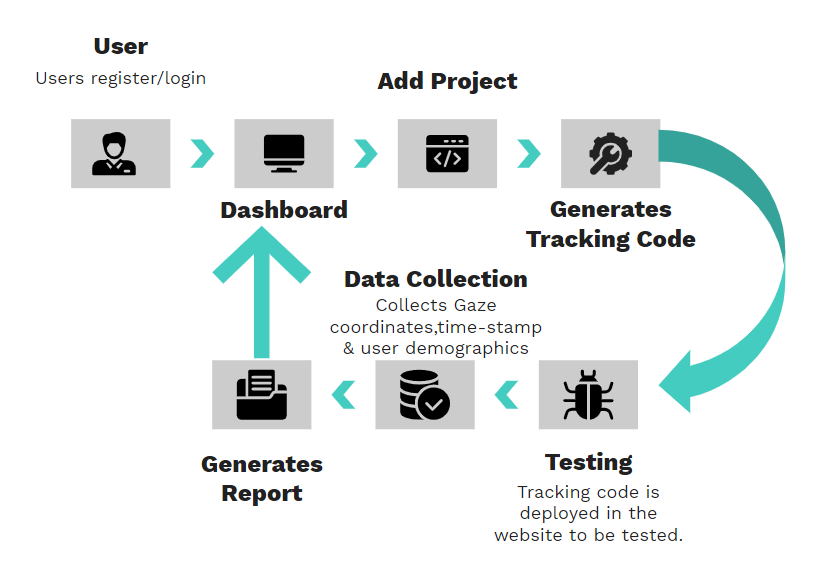
\includegraphics[width=\linewidth]{proposed-method.png}
    \counterwithin{figure}{section}
    \caption{Control Flow Diagram}
\end{figure}
The system mainly consist of 2 parts:
\begin{itemize}
	\item Client Side Script
	\item Backend \& Dashboard
\end{itemize}
\section{Website Tracking Script}
The client side script is a javascript file that performs the eye tracking calibration, eye tracking and user data collection. The script is also responsible to preload all the necessary dependencies including webgazer.js, jQuery and many more. To avoid the users from having to manually include each dependency and to prevent a dependency deadlock scenario, all the dependencies are packaged into a single script using webpack.

It mainly consist of the following modules:
\subsection{Tracking Code}
The tracking code is the only piece of code that a website manager needs to add to his/her site. A unique tracking code is generated for every project and the code is inserted into the \textbf{\textit{head}} tag of all the required webpages. The tracking code stores the unique variables of a project such as the project ID and other paramaters which can then be accessed from the tracking script.
\begin{figure}[H]
    \centering
    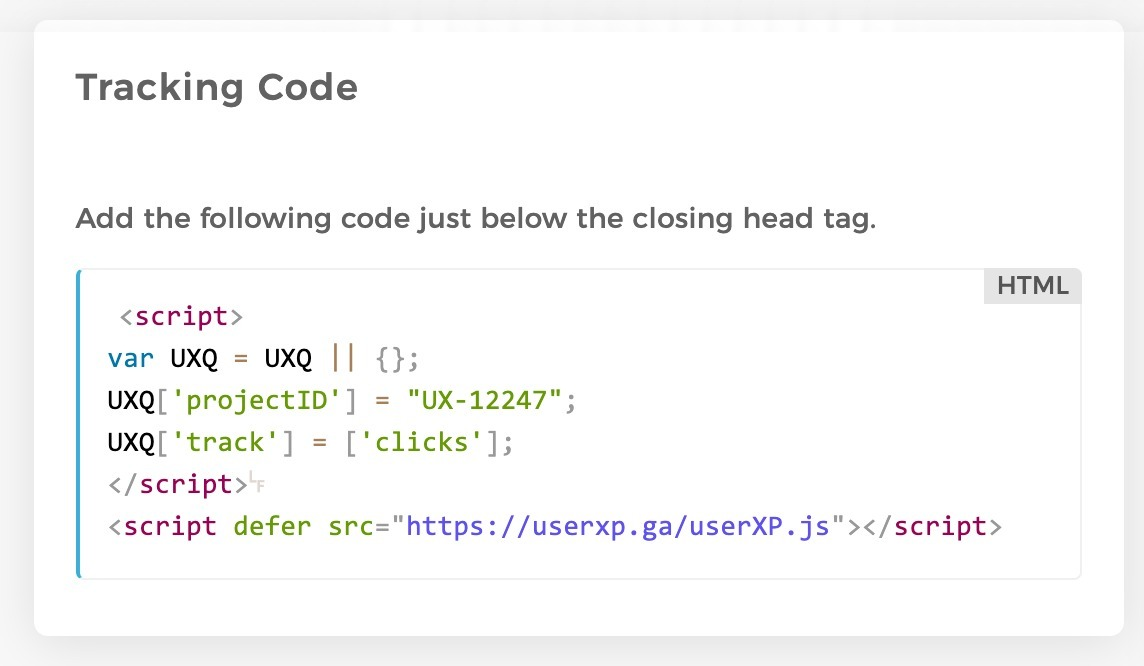
\includegraphics[width=\linewidth]{tracking-script.png}
    \counterwithin{figure}{section}
    \caption{Tracking Script}
\end{figure}

\subsection{Calibration \& Eye Tracking}
When the website to be tested is loaded it's content is replaced by the calibration page. During the calibration process the system learns how a tester’s eyes move when they are looking at certain parts of the screen.
WebGazer, a self callibrated eye-tracking library is used for obtaining the eye-gaze locations of varoius testers on the website in real time.

In the initial phase of calibration the eye tracking model is self callibrated by matching the pupil positions and eye features with screen locations during user interactions.
Upon completion the calibration page hides away revealing the website which the users can interact normally for the specified duration which is defaulted to 30 seconds. On hitting the specified time interval, a form appears and prompts the tester to submit his/her basic details such as age and gender. The tracking results are also submmited along with the form.
\begin{figure}[H]
    \centering
    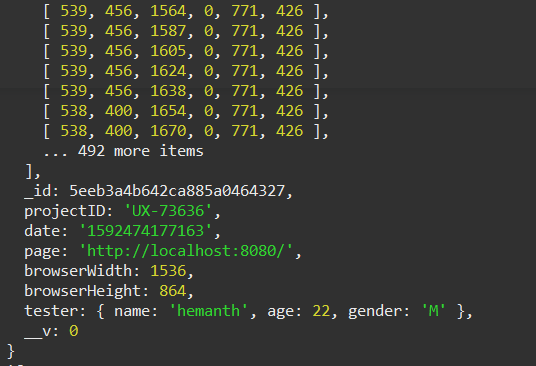
\includegraphics[width=\linewidth]{tracking-data.png}
    \counterwithin{figure}{section}
    \caption{Tracking Data}
\end{figure}

The above figure shows a snippet of the data being posted to the server after the test.
The submited data consist the following data:
\begin{itemize}
	\item Project ID: A unique ID to identify each project.
	\item URL: URL of the website to be tested.
	\item Browser Dimentions: It consist of the browser width and height in pixels.
	\item User Demographics: Details such as name, age and gender of the tester.
	\item Gaze-Recording: It consist of 5 attributes-Eye Coordinates(both x \& y coordinates), Timestamp, Scroll Offset and Mouse Coordinates(both x \& y coordinates) respectively.
\end{itemize}


\section{Dashboard}
It's an interactive website made using HTML,CSS \& JS which acts as platform for the users for adding, managing and the deletion of their projects.
Each of the projects page is equipped with various details such as tracking code, user demographic chart and the listing of all the testers along with the links to each report.

\subsection{Sign Up and Login}
The website manager can register in our platform by signing up with an email \& password or by using sign up using Google option.
\paragraph{}
With the regular sign up, a user can create an account with his/her email address and a password. The password is encrypted using MD5 encryption algorithm and the user details are stored into the database.
Users can also signup using their Google accounts, where basic details like name, email and image will be retrieved from Google and will be stored in our database. In the latter case no passwords are stored in our database unless added otherwise.

\subsection{Project Management}
Dashboard also acts as a platform where the users can create, update and delete projects. Once the user logs into the dashboard all his existing projects will be displayed. 
\subsubsection{Project Creation}
The prompt for creating a new project is shown below. In this the user have to enter the name of the project as required, the URL of the website to be tested and the maximum number of testers required for this project. Once the project is created, the above details are added into the database.
\begin{figure}[H]
    \centering
    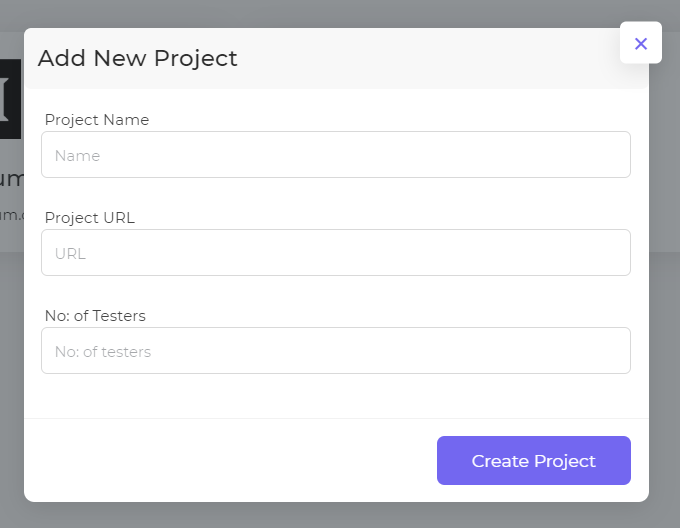
\includegraphics[scale=.8]{create-project.png}
    \counterwithin{figure}{section}
    \caption{Create new project prompt}
\end{figure}
\subsubsection{Project Details}
\begin{figure}[H]
    \centering
    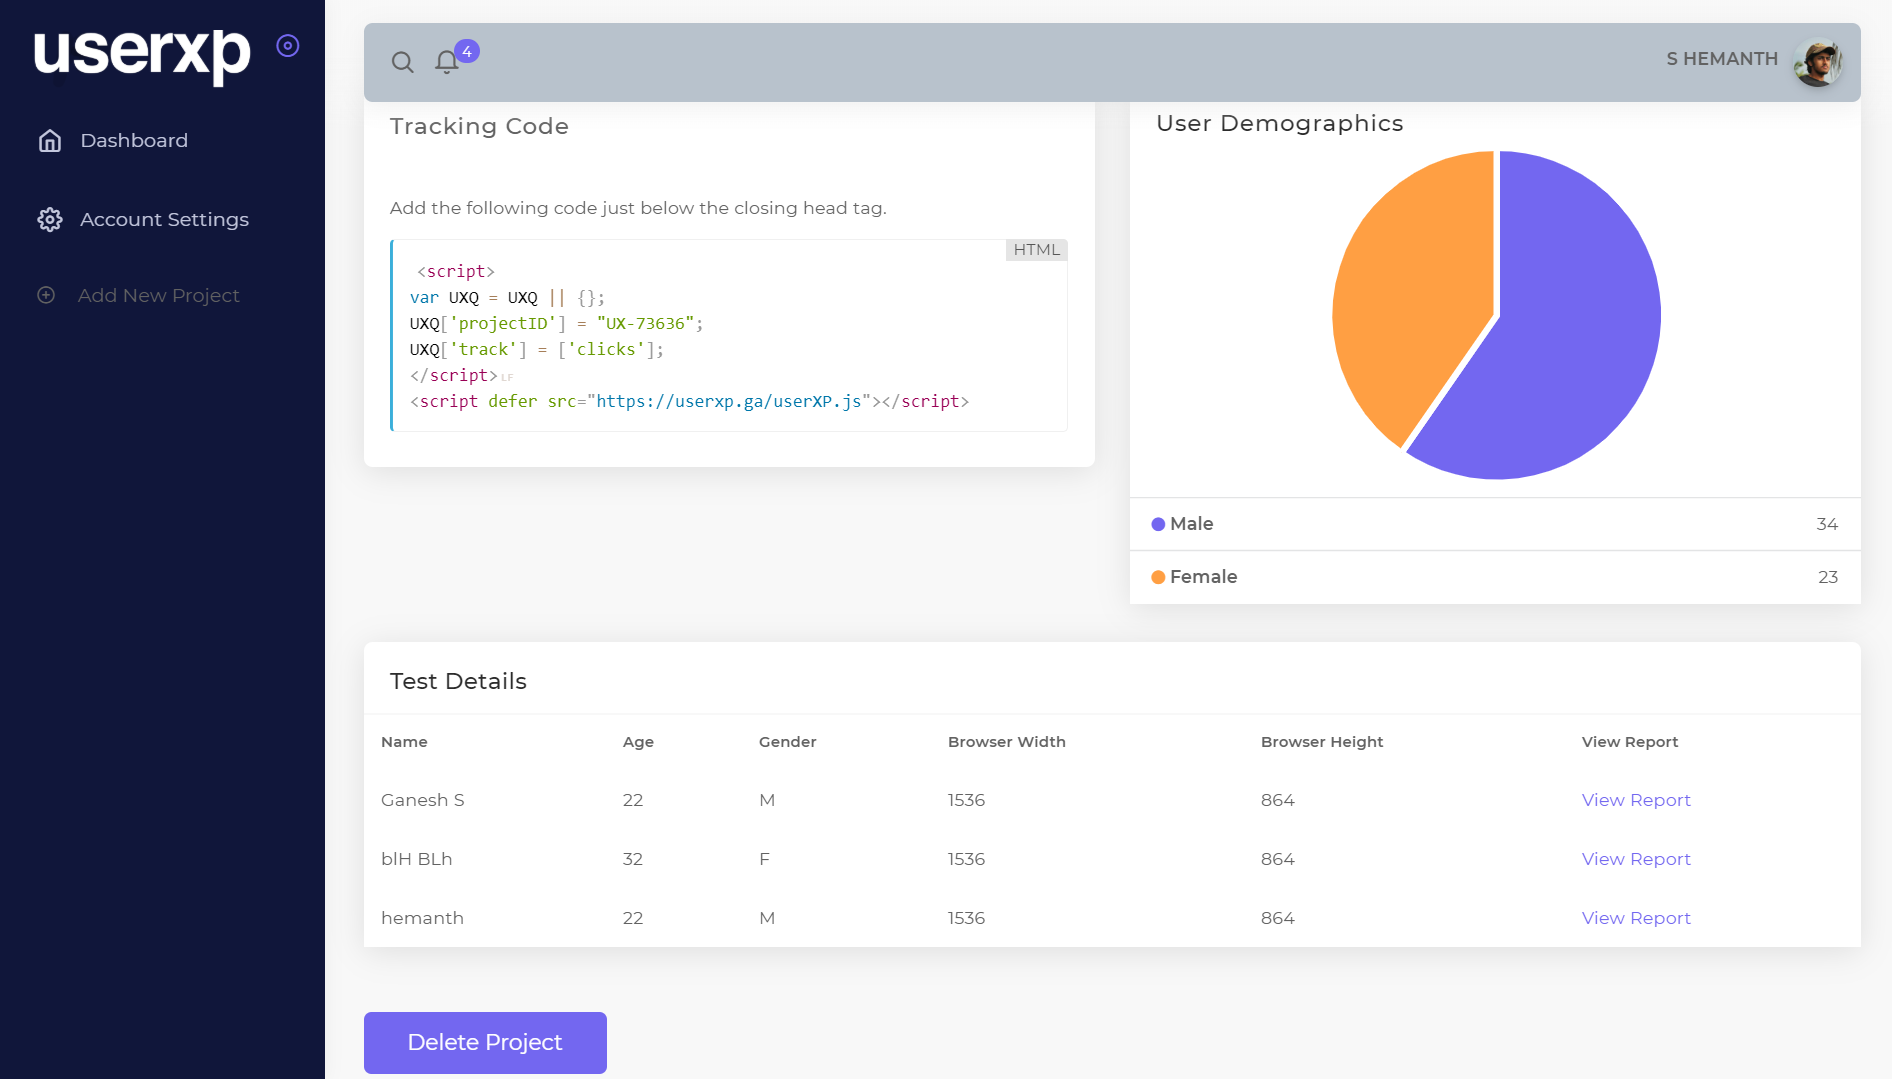
\includegraphics[width=\linewidth]{project-page.png}
    \counterwithin{figure}{section}
    \caption{Project Page}
\end{figure}
Each project page contains the unique tracking code for that project which is to be inserted into the website to be tested.
A pie-chart displaying the details of the tester demographics and a table showing the details of all the testers for this project along with their individual report.
An option to delete the project is also available. Once the project is deleted the project data along with the tester’s data is removed from the database.

In order to avoid the accidental deletion of the project, the user is asked to enter the Project-ID to confirm the deletion process.
\begin{figure}[H]
    \centering
    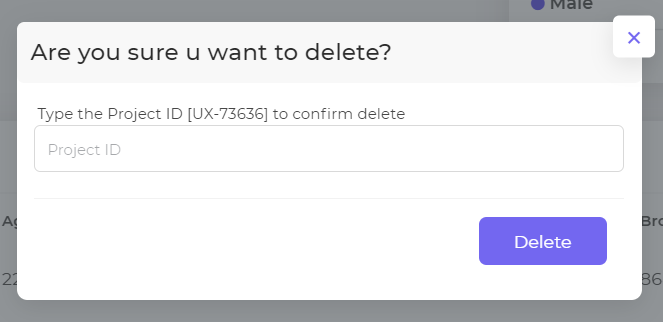
\includegraphics[scale=.8]{delete-project.png}
    \counterwithin{figure}{section}
    \caption{Delete Project Prompt}
\end{figure}

\newpage
\subsection{Usability Report and it's Features}
A usability report is generated from the data obtained from each testes of a project which provides an insight on how various testers interacts with the website and infer the necessary changes to be made so as to improve the user experience.

Various features of the report are:
\subsubsection{Heat map \& Gaze Opacity Map}
A heatmap is a visualization that uses different colors to highlight the regions viewed by the tester. Heat maps are color coded: red is typically used to indicate the most focused region and
green the least, with varying levels in between. An area with no color on a heat map signifies that the participants may not have focused on the area.
\begin{figure}[H]
    \centering
    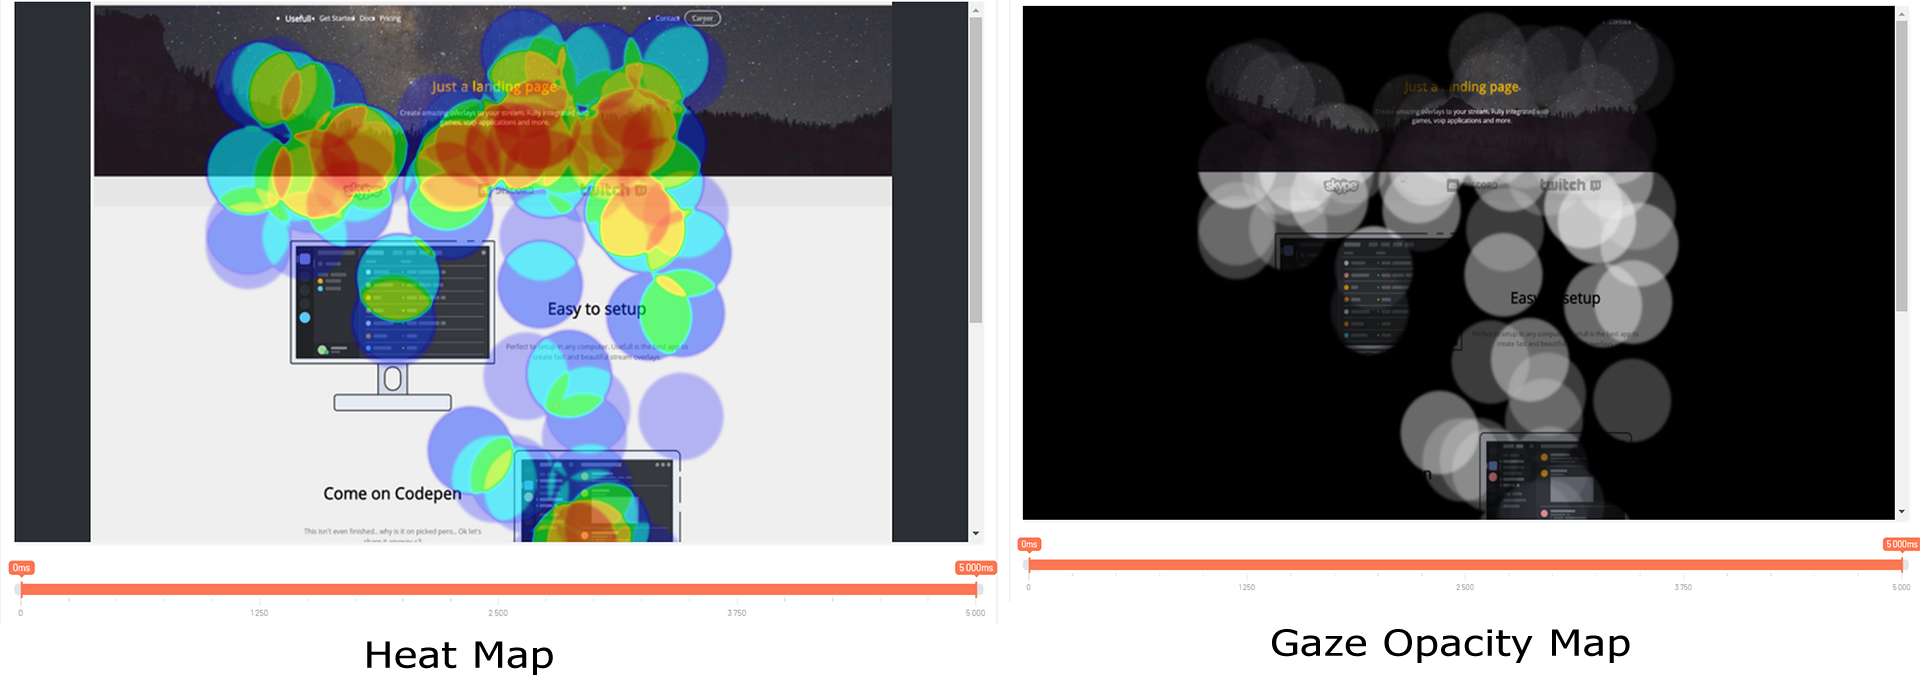
\includegraphics[width=\linewidth]{heat_gaze_map.png}
    \counterwithin{figure}{section}
    \caption{Heat Map \& Gaze Opacity Map}
\end{figure}
The Gaze Opacity map is an inverse map of compiled fixation data. The opposite of a heat map, it is best used to highlight
areas of user interaction on the website.The white region in this map marks the region where the tester had focused and the black region corresponds to less interaced area.
It is also known as a Spotlight map.
\subsubsection{Area of Interest(AOI)}
AOIs are specific areas or content of the user interface that
interests the UX team. The user can select any specific portion on the website by drawing a square box in the window and can obtaine the details on how much time the tester had spend in that region.
\begin{figure}[H]
    \centering
    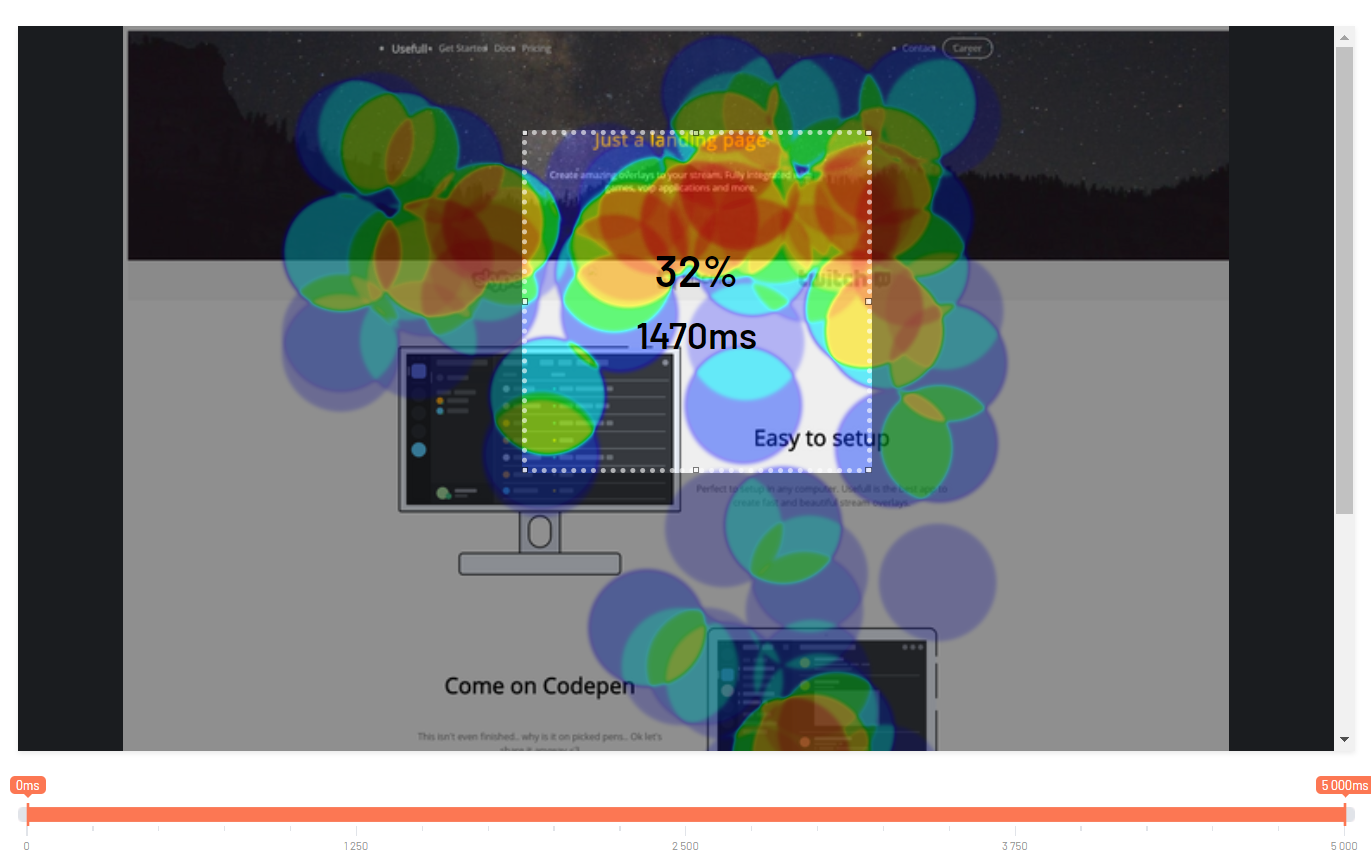
\includegraphics[width=\linewidth]{AOI.png}
    \counterwithin{figure}{section}
    \caption{Area of Intrest(AOI)}
\end{figure}
In the above figure,the square portion marks the Area of Intrest and the data present shows that the user had spent 32\% of the total time in this region and spend about 1470ms here.

\section{Backend}
The backend of our system is powered by NodeJS with Express and peforms the tasks such as database management, routing, templating, authentication and it also provides API endpoints for the frontend. 

NodeJS is a JavaScript runtime built on Chrome's V8 JavaScript engine. It was used due to its high performance and the due to the fact that client side script is written in javascript.

EJS or Embedded Javascript Templating is a simple templating engine used by NodeJS that lets you generate HTML markup with plain JavaScript.It can inject data into HTML template at the server side and produce the final HTML. It is used because of it's fast compilation and rendering property.

MongoDB is leading NoSQl, cross-platform, document oriented database that provides, high performance, high availability, and easy scalability. MongoDB works on concept of collection and document. The data is stored in BSON(Binary JSON) format in the form of key-value pair.

\subsection{Database}
MongoDB was used as database due to the nature of data being dealt with. MongoDB uses JSON-like documents with optional schemas. The entire project runs on a single document with 3 collections.

\begin{figure}[H]
    \centering
    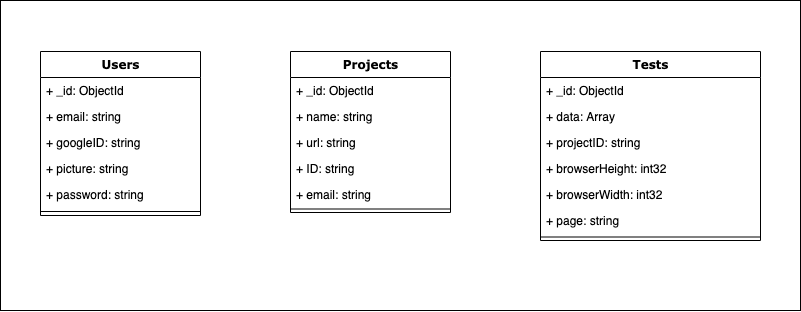
\includegraphics[width=\linewidth]{db.png}
    \counterwithin{figure}{section}
    \caption{MongoDB Collections}
\end{figure}
The figure shows the basic schema for the 3 collections but since MongoDB requires no schema we can easily add new entries to each document as a key-value pair.

\subsection{Authentication, Routing, Templating \& Other Tasks}
One of the first task of the backend is to authenticate users and we provide two methods for doing that. Users can signup using Google SSO or with an email and password. Authentication is handled by passportJS, a nodeJS library and users are authenticated with a cookie based approach.

\begin{figure}[H]
    \centering
    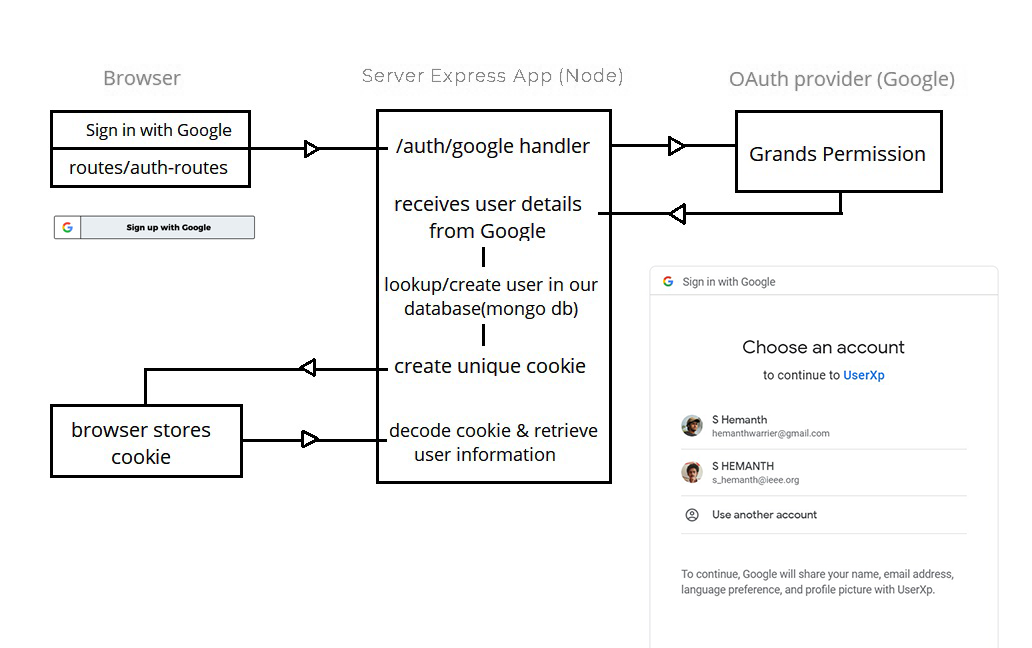
\includegraphics[width=\linewidth]{google-sso-auth.png}
    \counterwithin{figure}{section}
    \caption{Google SSO Authentication}
\end{figure}

Routes are defined using Express which is the goto framework for the purpose. It allows us to recieve and respond to different types of http requests like GET, POST or DELETE. 

Next, the backend generates the requested dashboard pages using EJS templating and is served as plain HTML files.

\subsection{API Endpoints}
The following APIs allow the frontend to interact with backend for CRUD operations.
\begin{itemize}
    \item \textbf{/api/v1/submit} This endpoint is used to recieve the form data from the website and it is available publically. To avoid misuse or false submissions, each request is verfied by crossmatching the origin URL and the URL in the database for the given project ID.
    \item \textbf{/api/v1/newProject} This endpoint should originate from an authenticated user and it creates a new DB entry with the given project details.
    \item \textbf{/api/v1/delete/:id} The delete endpoint takes an ID of the project which is to be deleted. The backend verifies that the request is coming from an authenticated user and also if the request originated from the corresponding project page. This ensures that other projects are not accidently or intentionally deleted by bruteforcing the id in the endpoint.
\end{itemize}
\subsection{Screenshot Module}
The final test reports require the screenshot of the website and for this we need a robust screenshot module capable of making screenshots at the given resolution. Though there are several screenshot APIs we decided to develop the module ourself. Screenshoting a website is a time consuming process and is CPU intensive thereby which we cannot add it into our existing pipeline in a synchronous manner as that may make the server unresponsive. So the module is developed such that it could be deployed separately and it can interact with the main server through APIs. Coordinating the screenshot jobs with the two systems can implemented with the help of job queues and task management systems like Kue. And as for the capturing the screenshot itself, we use Puppeteer, a Node library which provides a high-level API to control headless Chrome or Chromium. With Puppeteer we can launch a headless browser with the given width and height and generate the screenshot of the given website.
\subsection{Workflow}
\begin{figure}[H]
    \centering
    \includegraphics[width=\linewidth]{userXP- Workflow.png}
    \counterwithin{figure}{section}
    \caption{Workflow Diagram}
\end{figure}
\newpage
\chapter{LIMITATIONS \& FUTURE SCOPE}
\paragraph{}
Even an ambitious project like ours also comes with few hurdles. The goal of the proposed system is to provide a seamless experience to both the parties involved. However, it cannot be said fulfilled if the tester is restricted to use the website only for a given time period or if he/she is prevented from moving across pages. The former issue arises due to the storage and bandwidth constraints as a result of the sheer volume of the eye tracking data. Continuous steaming of tracking data through web socket connection seems to overcome the issue but is yet to be tested. 

The latter issue of not being able to browse through pages with eye tracking intact is also an indirect issue associated with browser storage limitations. 

Though webcam based eye tracking have immensely improved over the past few years, robust softwares that support major head movements are yet to be developed. Until then these computer generated reports should only be used as an aid than relying on it completely.

Finally, as privacy rights becomes stricter and data breaches becoming common we must be extra careful dealing with sensitive data.

As the technology extends to the general public, the essential concern of data privacy needs to be addressed. Eye data is valuable privacy-sensitive information that provides insight about human behavior, private life, health data, biometric signatures, etc. According to a survey conducted by Steil in 2019, people are interested in sharing eye-tracking data if it helps them in medical diagnosis or in improving their user experience but not for use in personal or behavioral study. This demands proper privacy regulations and changes in data capture mechanisms to protect user’s privacy.

\newpage
\chapter{CONCLUSION}
\paragraph{}
At present, existing Usability Testing methods for web based platforms are quite expensive and requires a considerable amount of resources including man-power and time.
\paragraph{}
\noindent 
We found that,

• Manual Testing requires more time or more resources, some times both

• Performance testing is impractical in manual testing.

• Less Accuracy

• Executing same tests again and again time taking process as well as Tedious.

• Not Suitable for Large scale projects and time bounded projects.

• Manual Test Case scope is very limited.

• Comparing large amount of data is impractical

\paragraph{}
Thus to overcome these challenges, the proposed system uses eye-tracking, cursor movement and mouse-clicks to evaluate the positions on the screen where the user pays more attention and records user activity to be analysed in reports. This testing is done for different age groups. A final analysis report is generated. The UX team in turn can use this report to identify what they have done right \& wrong and hence improve their design. 

So the users of this platform goes through easy steps to test and analyse results. Project created from the dashboard generates a tracking code for the users, which is then pasted on the source code of website/webpage to be tested.
When the testers arrive at the webpage to use it, a calliberation is run. Then after the website is used/tested, the tester must enter his basic data such as age, gender and name. The user, probably a UX designer can access the report of the tester from the UserXP project dashboard. 
UX designers require various data such as gaze points, area of interest of the users, heat maps etc to evaluate user's experience. So, we generate reports in heat-maps, area of interest graphs and timeline view. 
Also user demographics and personas define various other charectoral factors for the analysers. So the project dashboard provides demographics data and chart for them. 
\noindent
\paragraph{}
From using this platform a firm/organisation have many advantages over manual user testing such as,
\newline
1. Faster Feedback\newline
Improves communication among coders, designers, and Product Owners, and allows potential glitches to be immediately rectified
\newline2. Accelerated Results\newline
Plenty of time is saved even for intricate and enormous systems. This allows for the testing to be carried out repeatedly, delivering faster results each time with lesser effort and time.
\newline3. Reduced Business Expenses\newline
It contributes to a higher quality of work, thereby decreasing the necessity for fixing glitches after release and reduces project costs.
\newline4. Testing Efficiency Improvement\newline
Testing a website eventually take up significantly lesser amounts of time using this platform. 
\newline5. Thoroughness in Testing\newline
There is a guaranteed focus on all areas of testing, thereby assuring best possible quality.
\newline6. Faster Time-to-Market\newline
Test Automation greatly helps reduce the time-to-market of an application by allowing constant execution of tests. 


\newpage
\addcontentsline{toc}{chapter}{REFERENCES}
\vspace{0.3cm}
\begin{thebibliography}{}

    \bibitem{1}
    Chynal, Piotr \& Szymański, Jerzy (2011). \emph{Remote Usability Testing Using Eyetracking.}, \url{https://www.researchgate.net/publication/221053998_Remote_Usability_Testing_Using_Eyetracking}

    \bibitem{d}
    Agnieszka Bojko (2015). \emph{Eye Tracking in User Experience Testing: How to Make the Most of It}, \url{https://www.researchgate.net/publication/266161907_Eye_Tracking_in_User_Experience_Testing_How_to_Make_the_Most_of_It}

    \bibitem{d}
    Papoutsaki, Alexandra \& Sangkloy, Patsorn \& Laskey, James \& Daskalova, Nediyana \& Huang, Jeff \& Hays, James. (2016). \emph{WebGazer: Scalable Webcam Eye Tracking Using User Interactions.}, \url{https://jeffhuang.com/Final_WebGazer_IJCAI16.pdf}
    
    \bibitem{d}
    Jennifer Romano Bergstrom \& Andrew Jonathan Schall \emph{Eye Tracking in User Experience Design.}, \url{https://books.google.co.in/books?id=5Hp0AgAAQBAJ&lpg=PP1&ots=2Zh1X9Y9u0&dq=eye%20tracking%20in%20user%20experience%20design&lr&pg=PP1#v=onepage&q&f=false}

    \bibitem{d}
    Kiril Alexiev, Teodor Toshkov and Peter Dojnow. 2019. Accuracy and Precision of eye tracker by head movement compensation and calibration. \emph{20th International Conference on Computer Systems and Technologies (CompSysTech'19)}, Jun 21-22, 2019, Ruse, Bulgaria, 8 pages. \url{https://doi.org/10.1145/3345252.3345278.}

\end{thebibliography}

\end{document}
